\documentclass{assignment}
\ProjectInfos{光电子技术}{PHYS6651P}{2021-2022学年第一学期}{第九章作业}{}{陈稼霖}[https://github.com/Chen-Jialin]{SA21038052}

\begin{document}
\begin{prob}
    请说明光纤激光器的结构,它与光纤放大器的不同,以及光纤激光器和光纤放大器相比于传统器件有哪些优点.
\end{prob}
\begin{ans}
    光纤激光器的结构: 光纤激光器由激光介质和谐振腔组成, 其中激光介质为掺杂光纤, 谐振腔可由光纤端面上的镀膜或两端的定向耦合器构成.

    光纤激光器和放大器的区别: 光纤激光器有谐振腔结构, 而光纤放大器无谐振腔结构, 泵浦光通过定向耦合器耦合入掺杂光纤中.

    光纤激光器相对于传统激光器的优点:
    \begin{itemize}
        \item[(1)] \textbf{更高的转换效率, 更低的激光阈值}: 光纤既是激光介质, 又是光的导波介质, 故在单模状态下泵浦光和激光充分耦合, 从而转换效率很高, 又由于光纤的形状具有很低的体积/表面积比, 散热快, 损耗小, 因此光纤激光器的激光阈值很低.
        \item[(2)] \textbf{小巧灵活}: 光纤激光的谐振腔由端面的镀膜或两端的定向耦合器构成, 且光纤具有可挠性, 因此小巧灵活.
        \item[(3)] \textbf{更宽的调谐范围, 更好的单色性}: 作为激光介质的掺杂介质, 掺杂稀土粒子 (如 \ce{Nd^{3+}}, \ce{Er^{3+}} 等) 和承受掺杂的基质 (如硅化物玻璃、卤化物玻璃光纤等) 具有相当多的可调参数和选择性, 因此可获得的激光谱线相当多, 加之玻璃光纤的荧光谱相当宽, 插入适当的波长选择器等即可得到很宽的调谐范围和相当好的单色性.
    \end{itemize}

    光纤放大器相对于传统放大器的优点: 光纤放大器具有与光纤激光器相同的优点, 除此之外, 光纤放大器作为全光中继器代替光-电-光中继系统, 可以避免光-电、电-光转换过程中的遗失和差错, 减小时延, 结构简单, 造价低廉, 具有很高的可靠性.
\end{ans}

\begin{prob}
    利用光纤中的非线性偏振演变效应,设计出一种被动锁模光纤激光器系统,其系统如下
    \begin{figure}[H]
        \centering
        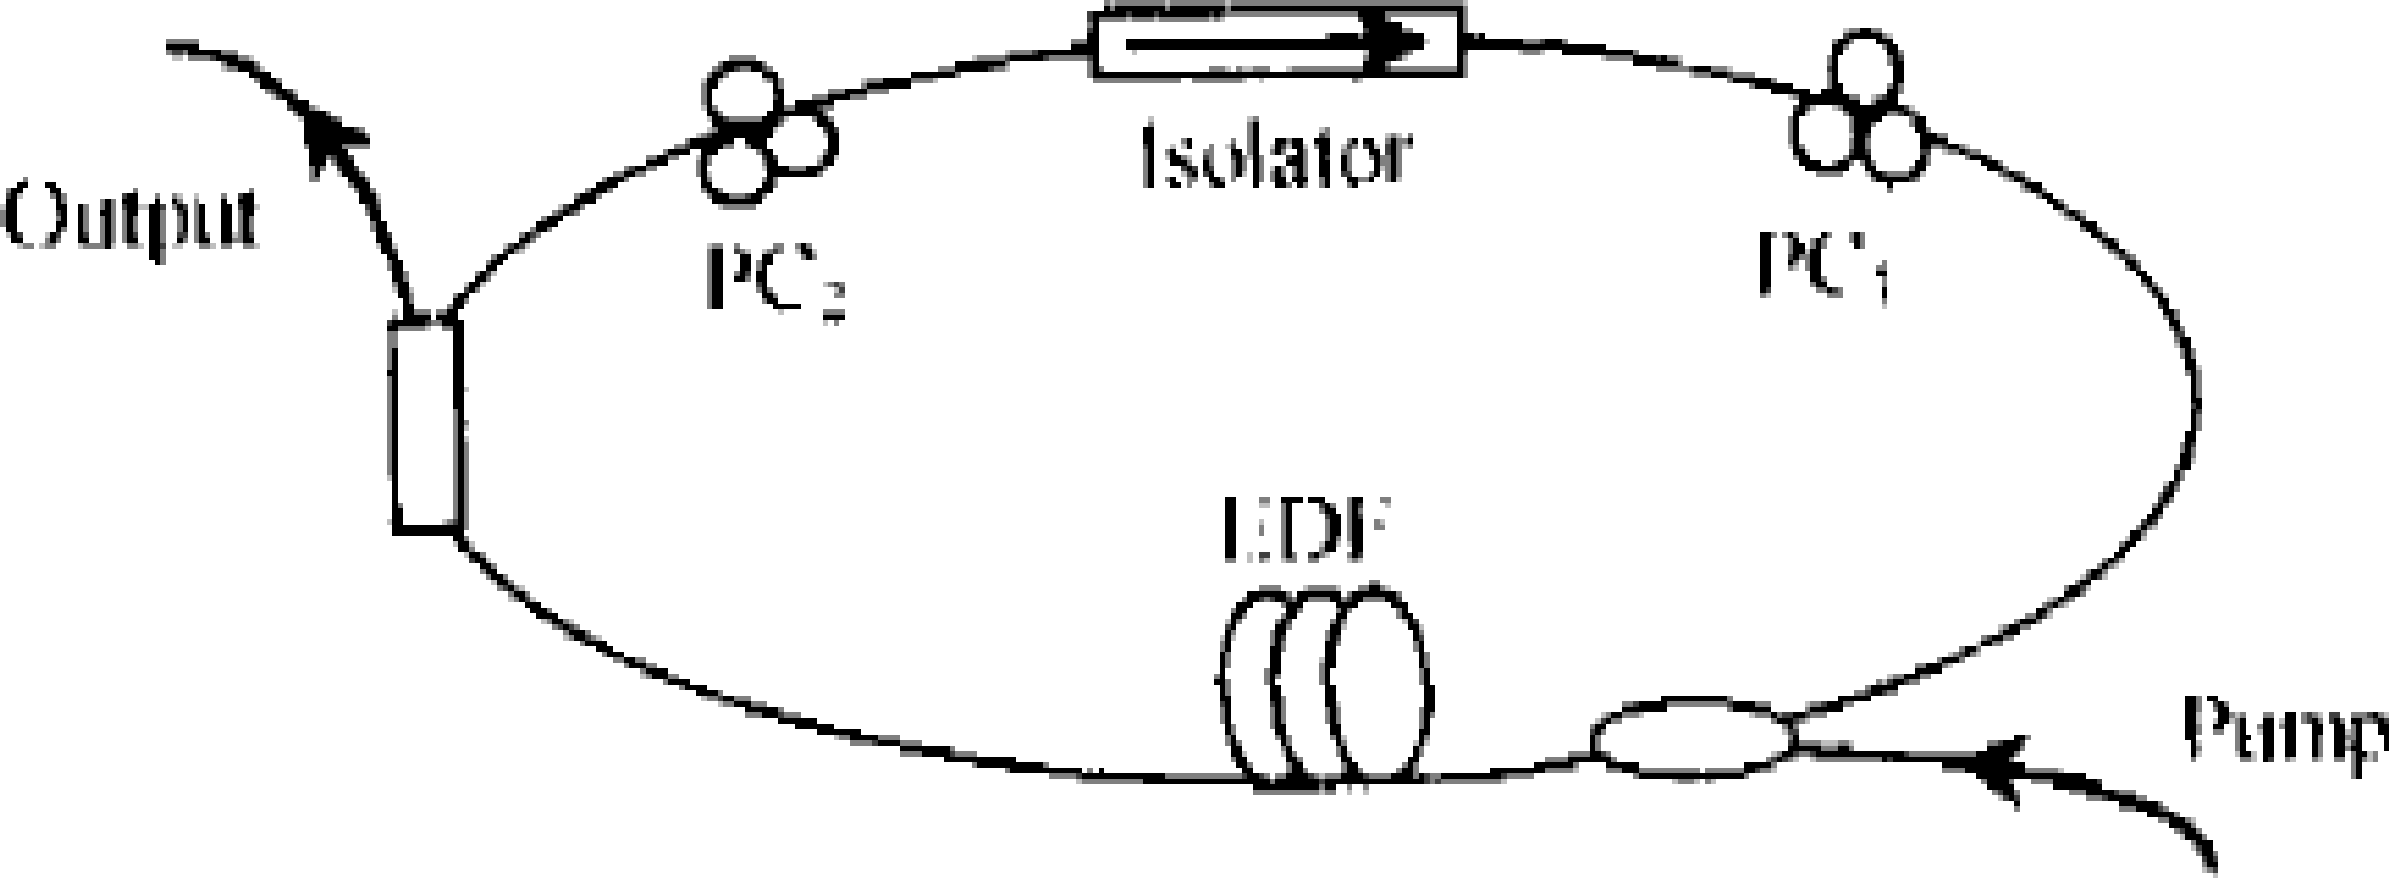
\includegraphics[width=.5\columnwidth]{5-1.png}
    \end{figure}
    PC1 和 PC2 是两块偏振控制器,试利用光纤中的偏振变化解释这种锁模光纤激光器的工作原理.
\end{prob}
\begin{ans}
    脉冲成型的初始阶段, 由噪声引起的幅度较小的信号光脉冲经过偏振敏感的隔离器后成为线偏振光, 线偏振光经过偏振控制器 PC1 后成为椭圆偏振光, 椭圆偏振光可分解为相互垂直的具有不同强度的偏振光. 由于非线性 Kerr 效应的作用, 不同强度的偏振光将积累不同的非线性相移, 相互垂直的线偏振光在偏振控制器 PC2 处重新合成椭圆偏振光时发生旋转.

    光脉冲的峰值处比前后沿积累更多的非线性相移, 通过调整 PC2, 使得光脉冲峰值处通过偏振敏感的光隔离器时损耗最小, 而光脉冲的前后沿被抑制, 从而实现光脉冲的窄化, 使激光器工作在锁模状态.
\end{ans}
\end{document}